%% LyX 2.1.1 created this file.  For more info, see http://www.lyx.org/.
%% Do not edit unless you really know what you are doing.
\documentclass[english]{article}
\usepackage[T1]{fontenc}
\usepackage[latin9]{inputenc}
\usepackage{color}
\usepackage{babel}
\usepackage{graphicx}
\usepackage[unicode=true]
 {hyperref}

\makeatletter

%%%%%%%%%%%%%%%%%%%%%%%%%%%%%% LyX specific LaTeX commands.
%% A simple dot to overcome graphicx limitations
\newcommand{\lyxdot}{.}


\makeatother

\begin{document}

\title{ATF35143 S-parameter extrapolation to low frequencies}

\maketitle
(Source code given in \href{file:https://github.com/pauluskruger/pauluskruger.github.io/tree/master/example3/Fetmodel}{example3/Fetmodel})


\section{HEMT Model}

The package model as given in the manufacture datasheet are used to
model the package and the following model is used to model the chip
(\href{file:Model.ckt}{Circuit}):

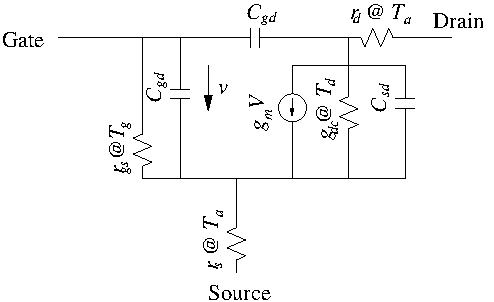
\includegraphics{hemt2}

The value of Ta = 290K is kept fixed and all other values of the chip
model are optimised \href{file:Model.ckt}{Model}.


\section{Fit results}

First the model is fitted to the S-parameters over the bandwidths
0.5-3~GHz (A) and 0.5-10~GHz (B).

The fitted values are \href{http://Model.dat}{A} and \href{http://ModelFull.dat}{B}
and the graphs below shows how the model compare to the S-parameters. 

A new \href{http://atf35143_M1.s2p}{S-Parameters} file is then generated
using the model, which is used in the amplifier design.

Graph Legend: \textcolor{red}{T1: Model A, }\textcolor{green}{T2:
Manufacturers S-Parameters, }\textcolor{blue}{T3: Model B}

\includegraphics[width=0.45\columnwidth]{Y11R\lyxdot txt}\includegraphics[width=0.45\columnwidth]{Y11I\lyxdot txt}

\includegraphics[width=0.45\columnwidth]{Y12R\lyxdot txt}\includegraphics[width=0.45\columnwidth]{Y12I\lyxdot txt}

\includegraphics[width=0.45\columnwidth]{Y21R\lyxdot txt}\includegraphics[width=0.45\columnwidth]{Y21I\lyxdot txt}

\includegraphics[width=0.45\columnwidth]{Y22R\lyxdot txt}\includegraphics[width=0.45\columnwidth]{Y22I\lyxdot txt}

\includegraphics[width=0.45\columnwidth]{NP1\lyxdot txt}\includegraphics[width=0.45\columnwidth]{NP2\lyxdot txt}

\includegraphics[width=0.45\columnwidth]{NP3\lyxdot txt}
\end{document}
